\chapter{Project Design}
\label{cha:design}
We implemented and tested the project in a real environment and also in simulation. WebRTC APIs are web browser APIs, meaning that they can only work in a browser session. So we developed a first version of the WPSS that works in the browser, and tested it with few nodes (100) using Google Chrome\footnote{Google Chrome is a free-ware web browser developed by Google} as browser. Then, in order to test it in a bigger environment we used a simulator. Both versions are implemented using the framework \textbf{Hivejs-Framework} provided by the creator of the algorithm, the Hive Streaming\footnote{Hive Streaming provides network solutions for media distribution and performance analysis. Started as a spin-off in 2007 from the Swedish Institute for Computer Science and the Royal Institute of Technology in Stockholm, the company maintains a strong focus on research and development. \url{https://www.hivestreaming.com}} company. This framework is written in Typescript\footnote{TypeScript is a typed superset of JavaScript that compiles to plain JavaScript. \url{http://www.typescriptlang.org}}, and it enabes us to choose if we want to run the project on browser or directly in \textit{Node.js} simulating a lot of instances. 


\section{Project Architecture}
\label{sec:arch}
At bootstrap-time, the node contacts the EasyRTC Server (Sect.~\ref{subsec:easyrtc_server}) to join the network. Then, it needs a way to build the base overlay with a fixed number of nodes, so it has to register itself to a tracker (Sect.~\ref{cha:tracker}), which it will return the list of the nodes that it has to contact. The tracker is also used to replace the broken links with new ones. In all the other cases, the peers communicate between each other without the help of an external server. The schema with all the steps is shown in Fig.~\ref{fig:project_architecture}.

\begin{figure}[ht]
  \centering
  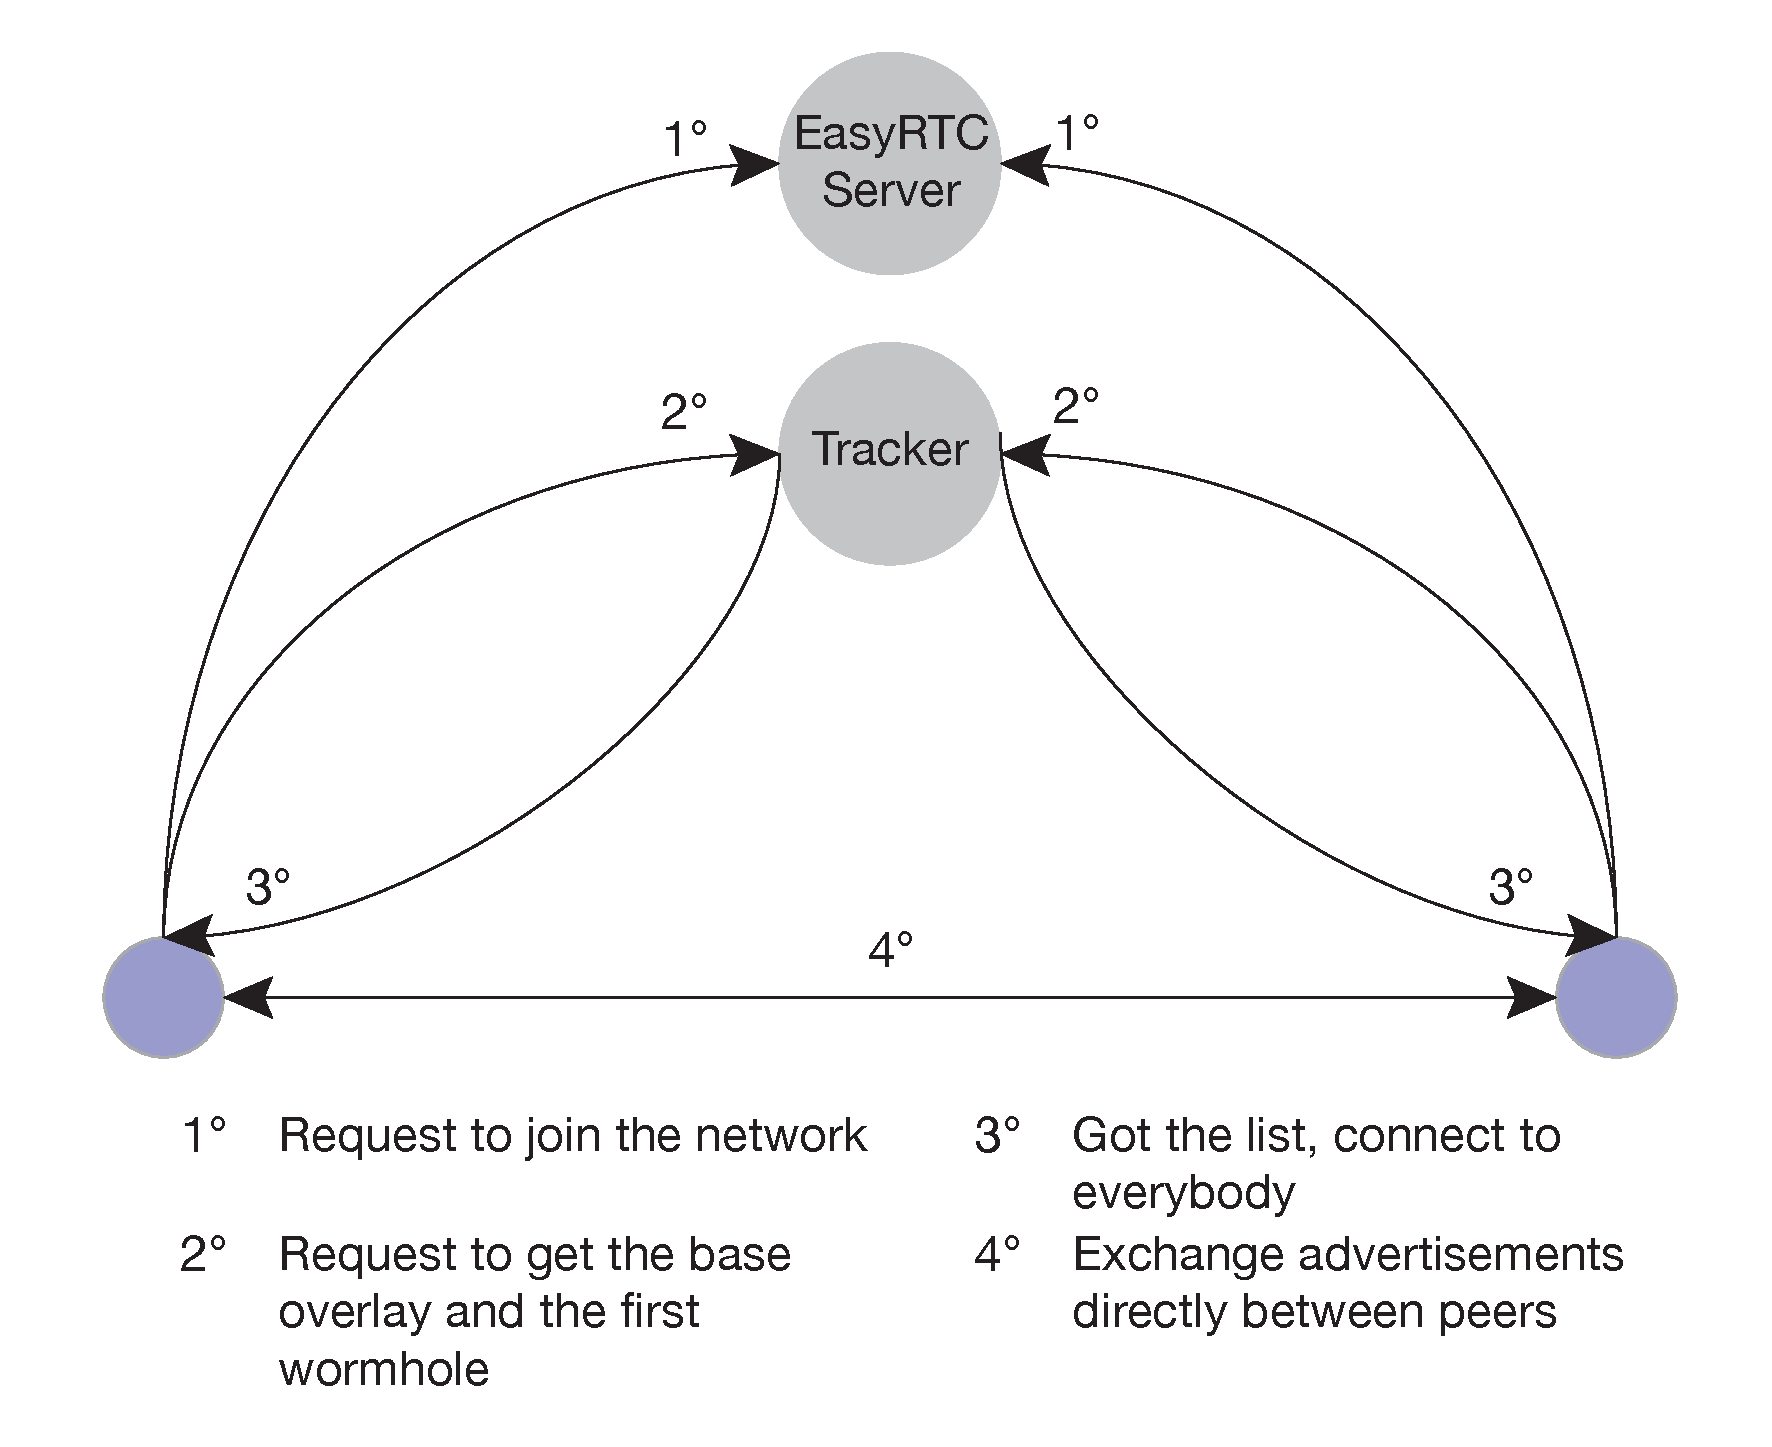
\includegraphics[keepaspectratio=true, width=\textwidth]{images/project_architecture}\caption{The architecture of the project, with the initial steps the nodes have to accomplish}
  \label{fig:project_architecture}
\end{figure}


\section{Node.js Modules}
\label{sec:modules}
The Hivejs-Framework has a WebRTC module for handling peer-to-peer connections which, as explained in Sect.\ref{sec:easy_tc}, is EasyRTC. Then we used a lot of other modules, the most important ones are:

\begin{itemize}
	\item \textbf{Browserify}: with browserify we can use some core \textit{Node.js} modules and many of the thousands modules on npm in our browser-side code
	\item \textbf{Grunt}: it is a task runner, we use it to compile, optimize and ``browserify'' our code. More information at \url{http://gruntjs.com}
	\item \textbf{Inversify}: Inversify is a lightweight (4KB) pico inversion of control (IoC) container for TypeScript and JavaScript applications
	\item \textbf{Q}: a library for promises, more information at \url{https://www.npmjs.com/package/q}
	\item \textbf{Fs}: we use this module only in simulation to write and save the logs of the nodes on local files.
\end{itemize}

The project in order to work correctly needs \textit{Node.js} version 0.12.5, \textit{npm} version 2.11.2 and \textit{Typescript} version 1.7.3.

\section{Special Tools}
We used a lot of tools to simplify the testing phase but also the implementation. One of the most important is NetworkX\footnote{\url{https://networkx.github.io}}, a Python language software package for the creation, manipulation, and study of the structure of complex networks. We used this tool to periodically draw the graphs of the network, in order to have a better representation of the overlays and to check the correctness of the implementation. 